% Twenty Seconds Resume/CV
% LaTeX Template
% Version 1.0 (14/7/16)
%
% Original author:
% Carmine Spagnuolo (cspagnuolo@unisa.it) with major modifications by 
% Vel (vel@LaTeXTemplates.com) and Harsh (harsh.gadgil@gmail.com)
%
% License:
% The MIT License (see included LICENSE file)
%
%%%%%%%%%%%%%%%%%%%%%%%%%%%%%%%%%%%%%%%%%

%----------------------------------------------------------------------------------------
%	PACKAGES AND OTHER DOCUMENT CONFIGURATIONS
%----------------------------------------------------------------------------------------
\newcommand{\wiesoich}{
    \textbf{Meine} praxiserprobten Kenntnisse in der Software-Entwicklung in C\#.Net,
    sowie meine langjährige Erfahrung in der\\ Analyse, Konzeption, Umsetzung und dem
    Testing individueller Lösungen, bringe ich ein fundiertes und \\praxiserprobtes
    Know-How mit.

    \textbf{Durch} meinen ausgeprägten und \\vielseitigen technischen Hintergrund,\\ meiner
    Kommunikationsfähigkeit und durch meine hohe Dienstleistungsmentalität
    kann ich im bestehenden Team, schnell \\ einen Mehrwert generieren.
}

\newcommand{\fromName}{Daniel Schmid}
\newcommand{\fromStreet}{Pergolastrasse 4}
\newcommand{\fromPlz}{3185}
\newcommand{\fromPlaceName}{Schmitten}
\newcommand{\fromPlace}{\fromPlz \hspace{1pt} \fromPlaceName}
\newcommand{\fromAdress}{ \fromName \\ \fromStreet \\ \fromPlace}
\newcommand{\fromDate}{\fromPlaceName, \today}
\newcommand{\fromTel}[1][078 771 55 22]{Tel: #1}


\newcommand{\toName}{ Intervista AG }
\newcommand{\toStreet}{ Optingenstrasse 5 }
\newcommand{\toPlace}{ 3013 Bern}
\newcommand{\toAdress}{ \toName  \\ \toStreet \\ \toPlace }
\newcommand{\goodbye}{Liebe Grüsse}
\newcommand{\letterSubject}{ }
\newcommand{\salutContact}{Lieber Christoph}
\newcommand{\letterText}{
    Anbei schicke ich dir den unterschriebenen Vertrag und mein Stammblatt zur Vervollständigung der Unterlagen zurück.
    
    Martin hat das Stammblatt bereits elektronisch erhalten.
}




\documentclass[a4paper]{twentysecondcv} % a4paper for A4

% Command for printing skill overview bubbles
\newcommand\skills{
~
\smartdiagram[bubble diagram]{
\textbf{~~~~Daniel~~~~}\\\textbf{~~~~Schmid~~~~},
\textbf{~~~~~~~~ruhig~~~~~~~~},
\textbf{pragmatisch},
\textbf{~~Teamgeist~~},
\textbf{~~~~~kreativ~~~~~},
\textbf{~analytisch~},
\textbf{~ziel~} - \\\textbf{~~orientiert~~}
}
}

% Programming skill bars
\programming{
{C $\textbullet$ C++  $\textbullet$ PHP $\textbullet$ Java / 2.5}, 
{Bash $\textbullet$ PowerShell $\textbullet$ \LaTeX / 3.5},
{HTML5 $\textbullet$ SASS / 4},
{C\#.Net $\textbullet$ MSSQL $\textbullet$ JS / 5}}

% Projects text
\projects{
\wiesoich
}

%----------------------------------------------------------------------------------------
%	 PERSONAL INFORMATION
%----------------------------------------------------------------------------------------
% If you don't need one or more of the below, just remove the content leaving the command, e.g. \cvnumberphone{}

\cvname{\fromName} % Your name
\cvjobtitle{ Full Stack Entwickler } % Job
% title/career

\cvlinkedin{/in/schmid-daniel/}
\cvgithub{}
\cvnumberphone{078 771 55 22} % Phone number
%\cvsite{daenu-schmid.ch} % Personal website
\cvsite{}
\cvmail{daenu.schmid@gmail.com} % Email address

%----------------------------------------------------------------------------------------

\begin{document}

    \makeprofile % Print the sidebar
    \hypertarget{work_back}{}
    \section{Berufliche Tätigkeit}
    \begin{twenty}
        \twentyitem
        {seit 2010}
        {}
        {Link Institut AG \textnormal{Luzern}}
        {\hyperlink{link}{\textcolor{pblue}{Zwischenzeugnis}}}
        {Spezialist IT Entwicklung}
        {\begin{itemize}
             \item Hauptverantwortlich für die Umsetzung eines neuen Befragungsfrontend in C\#.Net.
             \item Technische Hauptverantwortung für die Weiterentwicklung des LINK Internet-Panels
             (Verwaltungssoftware,Datenbank,Prozesse)
             \item Eigenständige Analyse, Konzeption und Planung von neuen Entwicklungsprojekten oder (Teil)-Projekten.
             \item Konzeption und Umsetzung von Java-Script Modulen, im Sinne neuer Fragetypen für Online-Umfragen.
             \item Weiterentwicklung und Wartung bestehender C̣\#/.Net-Applikationen (Windows-Services,Web-API's,Desktop Applikationen und Websites)
             \item Studienspezifische Entwicklungen komplexer Online Studien.
             \item Allgemeine Wartungsaufgaben (MS-SQL und MySql-Datenbanken, Anwendungen)
             \item Aufbau und Unterhalt der LINK-Subversion Umgebung
        \end{itemize}}
        \hypertarget{datahouse_back}{}
        \twentyitem        
        {}
        {}
        {}
        {}
        {}
        {}
  
        \twentyitem
        {2009 - 2010}
        {}
        {Datahouse AG \textnormal{Zürich}}
        {\hyperlink{datahouse}{\textcolor{pblue}{Arbeitszeugnis}}}
        {Applikationsentwickler}
        {
        \begin{itemize}
            \item Entwicklung von Webapplikationen in PHP
            \item Implementation von SOAP-Web-Services in C++
            \item Erstellung verschiedener Templates in \LaTeX
        \end{itemize}
        }
        \hypertarget{job_first_back}{}
        \twentyitem
        {}
        {}
        {}
        {}
        {}
        {}
        \twentyitem
        {2008 - 2009}
        {}
        {Jordi AG \textnormal{Schlieren}}
        {\hyperlink{jordi}{\textcolor{pblue}{Arbeitszeugnis}}}
        {Bereich: Mikroprozessorprogrammierung}
        {}
        \twentyitem
        {2006 - 2007}
        {}
        {T-Systems Schweiz AG \textnormal{Zollikofen}}
        {\hyperlink{tsystems}{\textcolor{pblue}{Arbeitszeugnis}}}
        {}
        {}
        \twentyitem
        {2005}
        {}
        {Bundesamt für Sozialversicherung \textnormal{Bern}}
        {\hyperlink{bsv}{\textcolor{pblue}{Arbeitszeugnis}}}
        {Berufspraktikum als Sachbearbeiter}
        {}

        \twentyitem
        {2004}
        {}
        {Booktrading,\textnormal{Freiburg}}
        {\hyperlink{booktrading}{\textcolor{pblue}{Arbeitszeugnis}}}
        {Berufspraktikum als Sachbearbeiter Buchhaltung}
        {}
        \twentyitem
        {2003}
        {}
        {WABCO (Schweiz) GmbH \textnormal{Bern Bümpliz}}
        {\hyperlink{wabco}{\textcolor{pblue}{Arbeitszeugnis}}}
        {Sachbearbeiter Betriebsbuchhaltung/Reporting}
        {}
    \end{twenty}
    %----------------------------------------------------------------------------------------
    %	 EDUCATION
    %----------------------------------------------------------------------------------------
    \hypertarget{cert_back}{}
    \section{Ausbildung}
    \begin{twenty} % Environment for a list with descriptions
        \twentyitem
        {seit 2019}
        {}
        {MCSA Lehrgang \textnormal{Zürich}}
        {}
        {}
        {}
        \twentyitem
        {2007 - 2009}
        {}
        {Informatikumschulung}
        {\hyperlink{informatik}{\textcolor{pblue}{Diplom}}}
        {Fachrichtung Applikationsentwicklung}
        {}
        \twentyitem
        {2005}
        {}
        {Cobol Programmierkurs \textnormal{Zürich}}
        {\hyperlink{cobol}{\textcolor{pblue}{Zertifikat}}}
        {}
        {}
        \twentyitem
        {2004}
        {}
        {Englischintensivkurs beim WSI \textnormal{Freiburg}}
        {\hyperlink{toeic}{\textcolor{pblue}{Zertifikat}}}
        {}
        {}
        \twentyitem
        {2000 - 2003}
        {}
        {Wirtschafts- und Kaderschule \textnormal{KV Bern}}
        {\hyperlink{kv}{\textcolor{pblue}{Diplom}}}
        {}
        {}
        \twentyitem
        {2000 - 2003}
        {}
        {WABCO (Schweiz) GmbH \textnormal{Bern Bümpliz}}
        {}
        {Kaufmännische Lehre}
        {}	%\twentyitem{<dates>}{<title>}{<organization>}{<location>}{<description>}
    \end{twenty}
    %----------------------------------------------------------------------------------------
    %	 EXPERIENCE
    %----------------------------------------------------------------------------------------

    \section{Referenzen}

    \begin{twenty} % Environment for a list with descriptions
        \twentyitem
        {auf Anfrage}
        {}
        {}
        {}
        {}
        {}
        %\twentyitem{<dates>}{<title>}{<location>}{<description>}
    \end{twenty}
    \newpage
    \hypertarget{link}{}
    
\includepdf[pages={1},scale=1,%
    picturecommand*={%
    \put(16,800){\hyperlink{work_back}{\textcolor{pblue}{zurück}}}%
    }]{cert/19_link.pdf}
    
\includepdf[pages={2},scale=1]{cert/19_link.pdf}
    \hypertarget{datahouse}{}
    
\includepdf[pages={1},scale=1,%
    picturecommand*={%
    \put(16,800){\hyperlink{datahouse_back}{\textcolor{pblue}{zurück}}}%
    }]{cert/10_datahouse.pdf}
    \hypertarget{jordi}{}
    
\includepdf[pages={1},scale=1,%
    picturecommand*={%
    \put(16,800){\hyperlink{job_first_back}{\textcolor{pblue}{zurück}}}%
    }]{cert/09_jordi_ag.pdf}
    \hypertarget{tsystems}{}
    
\includepdf[pages={1},scale=1,%
    picturecommand*={%
    \put(16,800){\hyperlink{job_first_back}{\textcolor{pblue}{zurück}}}%
    }]{cert/07_t_systems.pdf}
    \hypertarget{bsv}{}
    
\includepdf[pages={1},scale=1,%
    picturecommand*={%
    \put(16,800){\hyperlink{job_first_back}{\textcolor{pblue}{zurück}}}%
    }]{cert/05_bsv.pdf}
    
\includepdf[pages={2},scale=1]{cert/05_bsv.pdf}
    \hypertarget{booktrading}{}
    
\includepdf[pages={1},scale=1,%
    picturecommand*={%
    \put(16,800){\hyperlink{job_first_back}{\textcolor{pblue}{zurück}}}%
    }]{cert/04_booktrading.pdf}
    \hypertarget{wabco}{}
    
\includepdf[pages={1},scale=1,%
    picturecommand*={%
    \put(16,800){\hyperlink{job_first_back}{\textcolor{pblue}{zurück}}}%
    }]{cert/03_wabco-crop.pdf}
    \hypertarget{informatik}{}
    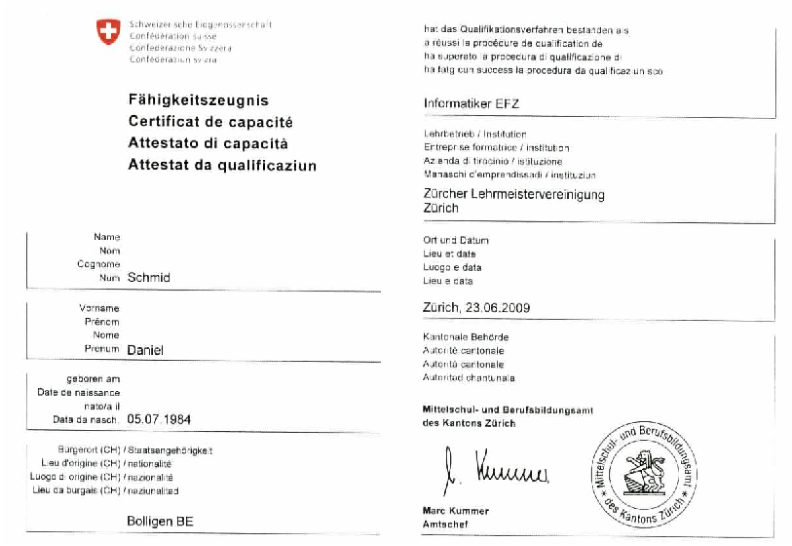
\includepdf[pages={1},scale=1,%
    picturecommand*={%
    \put(16,800){\hyperlink{cert_back}{\textcolor{pblue}{zurück}}}%
    }]{cert/09_informatiker.pdf}
    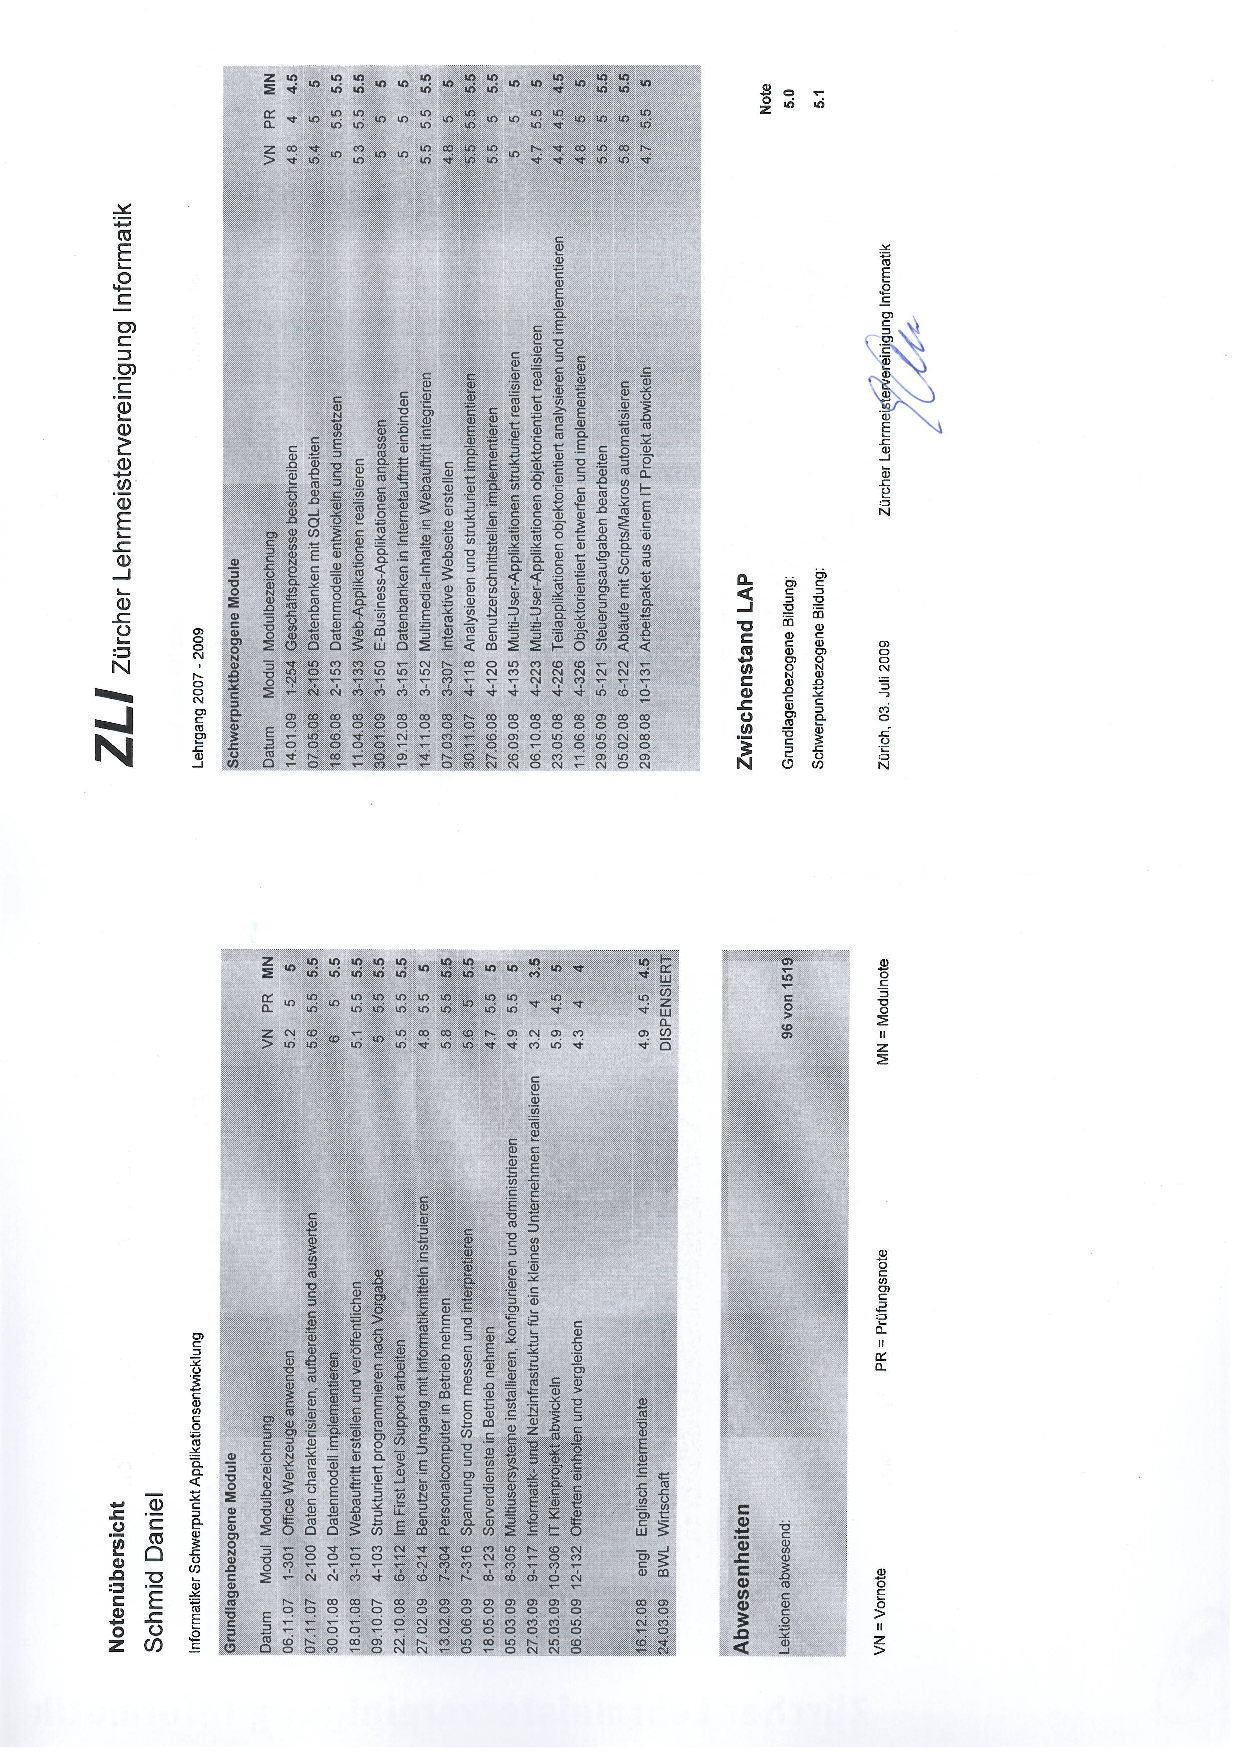
\includepdf[pages={1},scale=1,%
    picturecommand*={%
    \put(16,800){\hyperlink{cert_back}{\textcolor{pblue}{zurück}}}%
    }]{cert/09_cert_informatik.pdf}
    \hypertarget{cobol}{}
    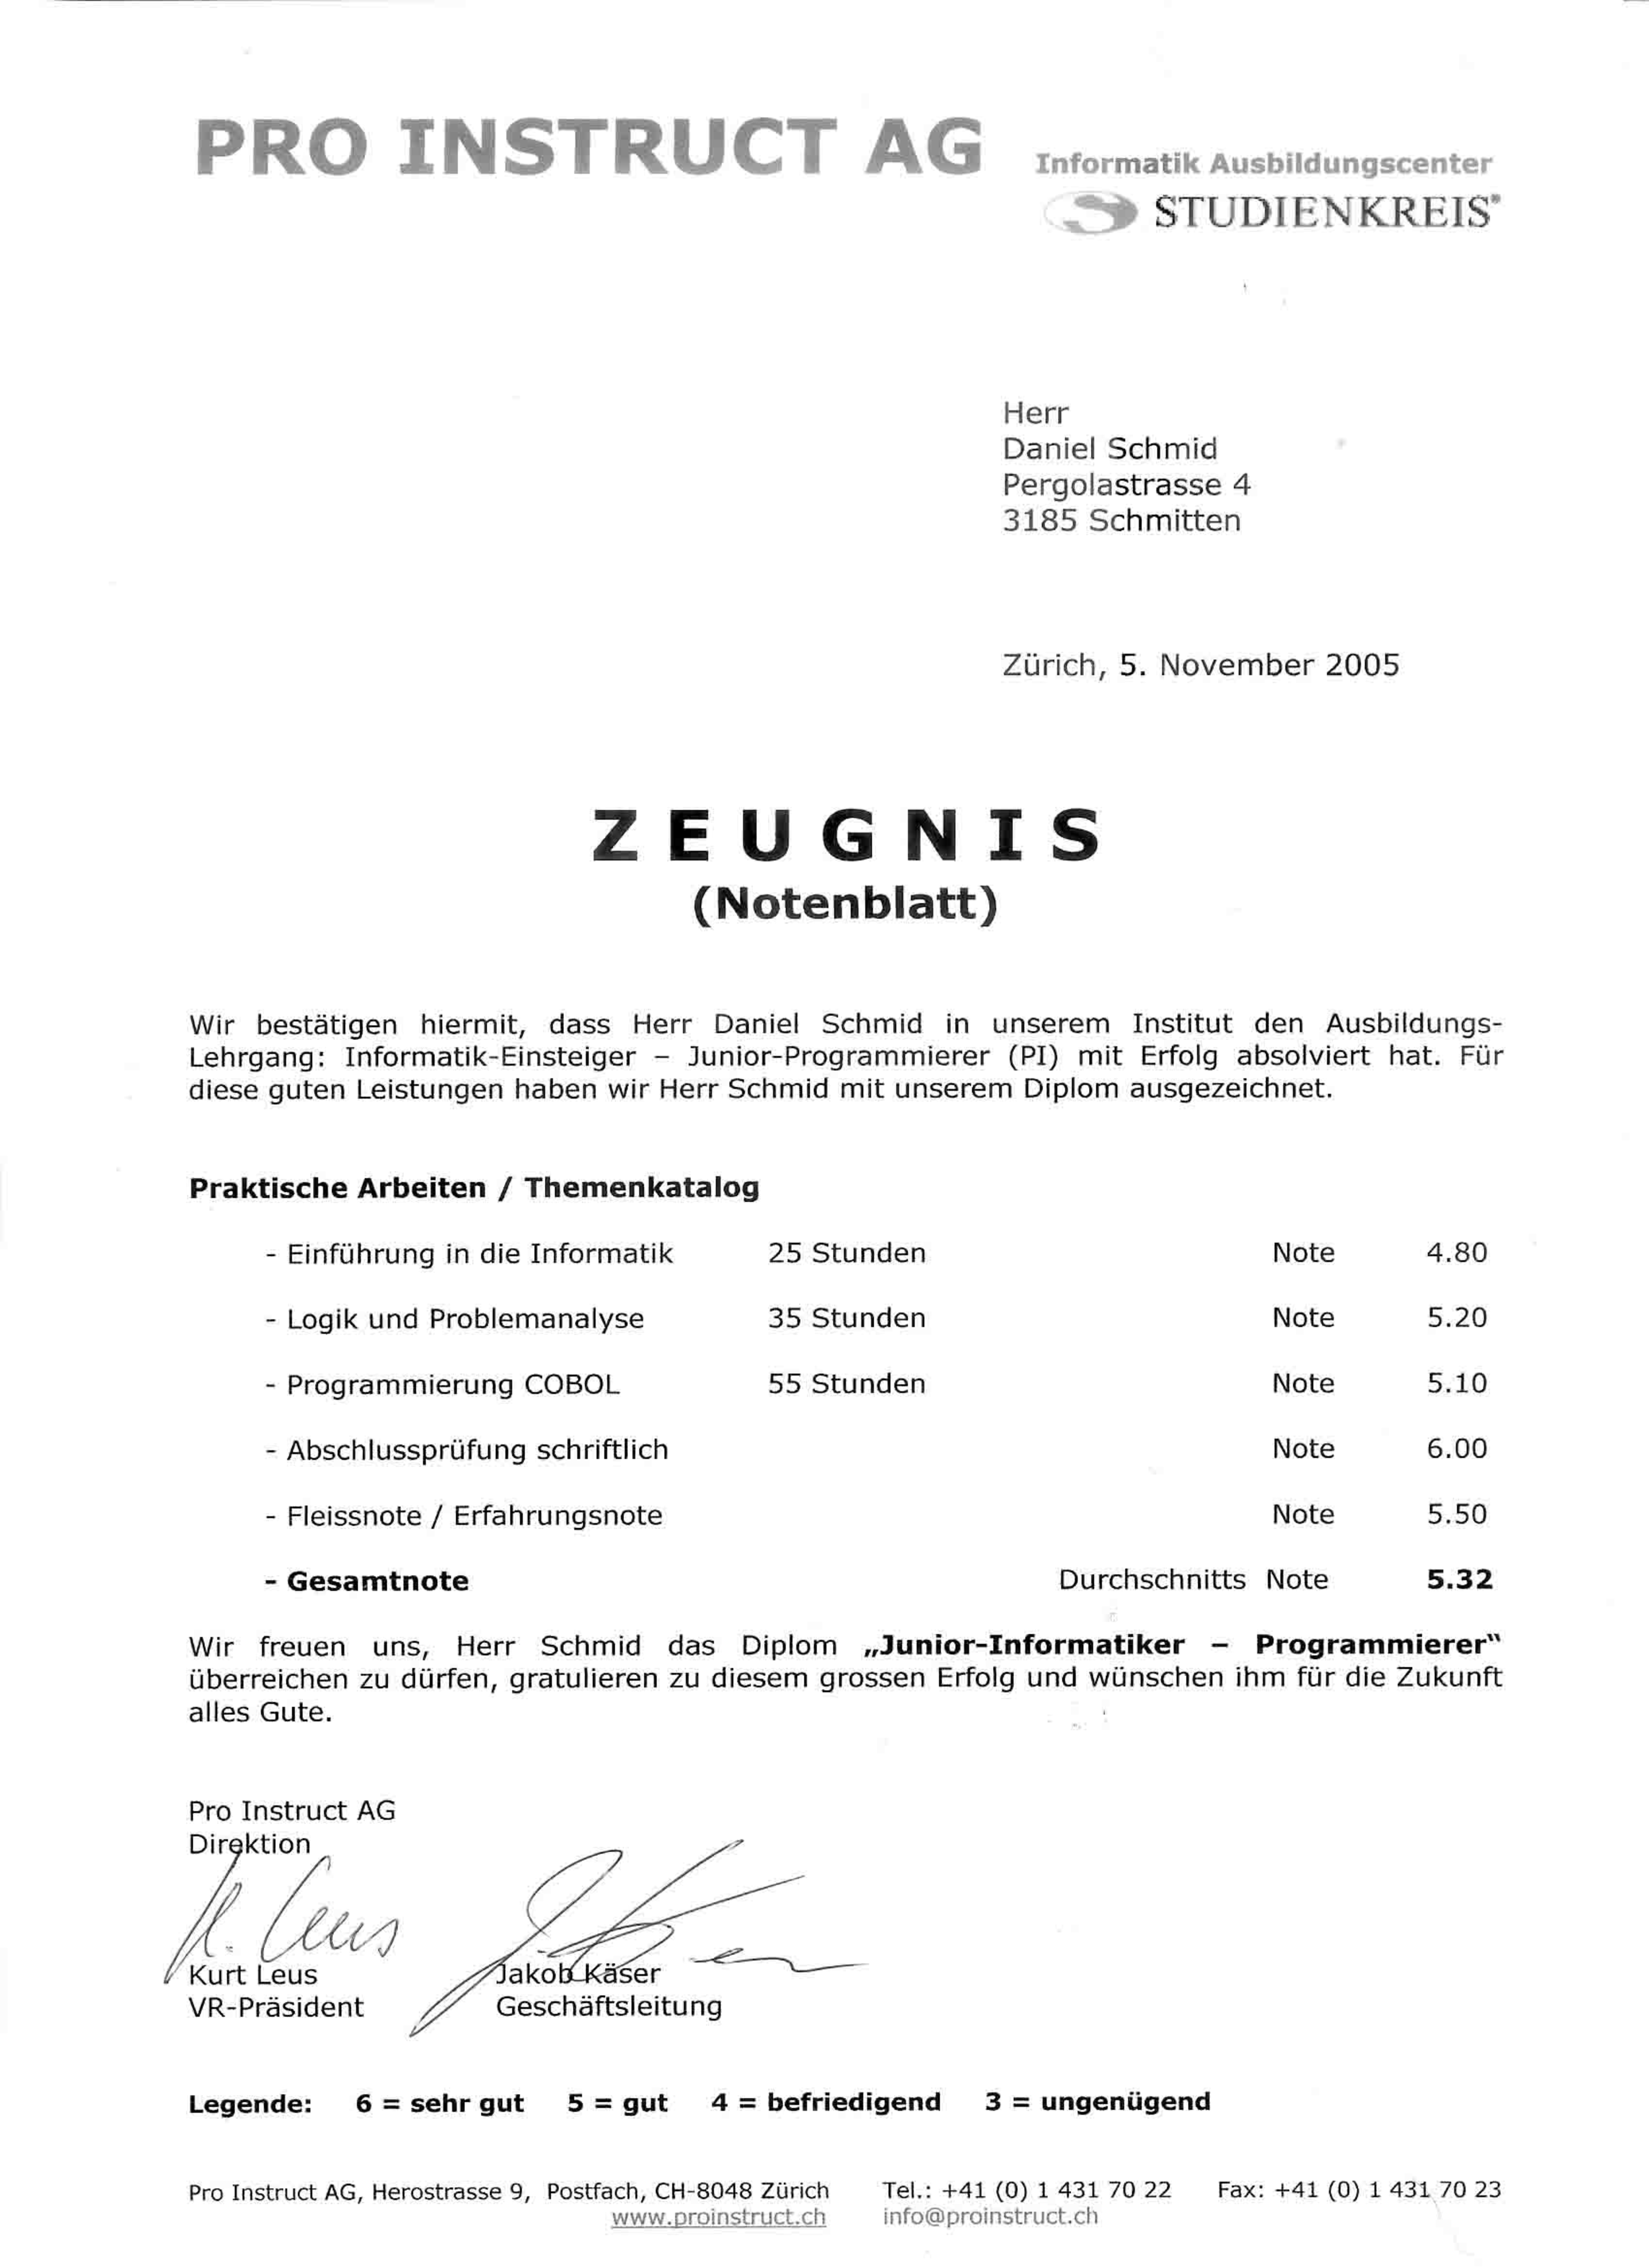
\includepdf[pages={1},scale=1,%
    picturecommand*={%
    \put(16,800){\hyperlink{cert_back}{\textcolor{pblue}{zurück}}}%
    }]{cert/05_course_cobol.pdf}
    \hypertarget{toeic}{}
    
\includepdf[pages={1},scale=1,%
    picturecommand*={%
    \put(16,800){\hyperlink{cert_back}{\textcolor{pblue}{zurück}}}%
    }]{cert/05_toeic.pdf}
    \hypertarget{kv}{}
    
\includepdf[pages={1},scale=1,%
    picturecommand*={%
    \put(16,800){\hyperlink{cert_back}{\textcolor{pblue}{zurück}}}%
    }]{cert/03_cert_kv.pdf}
    %\hypertarget{siz}{}
    %
\includepdf[pages={1},scale=1,%
    %	picturecommand*={%
    %	\put(16,800){\hyperlink{cert_back}{\textcolor{pblue}{zurück}}}%
    %}]{cert/02_course_siz.pdf}
\end{document} 
